% 05_results -- paper-results lane. Numbers: \res macros from generated/numbers.tex (figures/make_figures.py),
% generated tables (tables/res_*.tex), or a % src: comment.
\section{Results}\label{sec:results}

Unless stated otherwise, every method is scored on the 2,656 \Deb{} eval units with the same scorer;
invalid outputs count as wrong, and brackets are 95\% family-cluster bootstrap CIs
over the 42 families~\cite{efron1979}.
DeepSeek runs on \Dead, \Plac{} and \Orig{} cover the nested25 subset (\res{x}{n_nested25} units, paired).

\subsection{RQ1: Is the benchmark measuring leaks?}\label{sec:rq1}

Table~\ref{tab:probes} shows that original Juliet can be solved without looking at memory.
On \Orig, the string \code{static void} separates good from bad perfectly
(\res{x}{probe_static_void_original}),
and a function-count rule reaches \res{x}{probe_func_count_original}.
Debiasing removes these template cues: on \Deb{} both fall to chance
(\res{x}{probe_static_void_layer1} and \res{x}{probe_func_count_layer1}).
What remains is the free itself.
A bag-of-words model still scores \res{x}{probe_bow_lr_layer1} on \Deb,
because a unit without any \code{free}/\code{delete} is almost always a leak;
only on \Dead, where both labels contain the same number of frees, does it drop to \res{x}{probe_bow_lr_layer3}.

% generated by figures/make_figures.py -- do not edit
% src: juliet_full/analysis/score.py on original/ and layer1/ runs listed in generated/results_summary.json; probe row: juliet_full/data/build/probes_layer3.json
\begin{table}[t]
\centering
\caption{Every method on original Juliet (\Orig) and on our debiased units (\Deb), macro-F1 on the same eval units. $\Delta$ = \Deb{} $-$ \Orig. $^\dagger$DeepSeek: nested25 subset (664 units). Dynamic tools are a reference, not ranked.}
\label{tab:orig}
\scriptsize
\setlength{\tabcolsep}{4pt}
\begin{tabular}{@{}lrrr@{}}
\toprule
Detector & \Orig{} & \Deb{} & $\Delta$ \\
\midrule
probe: \code{static void} $\Rightarrow$ good & 1.000 & 0.333 & $-$0.667 \\
DeepSeek L1$^\dagger$ & 0.961 & 0.998 & +0.038 \\
Jev L1 & 0.956 & 0.971 & +0.015 \\
ASan/LSan (ref.) & 0.945 & 0.945 & $\pm$0.000 \\
LoRA L1 & 0.943 & 0.984 & +0.041 \\
grep (no \code{free}/\code{delete} $\Rightarrow$ leak) & 0.935 & 0.701 & $-$0.233 \\
Clang SA & 0.822 & 0.855 & +0.033 \\
CodeQL & 0.785 & 0.882 & +0.097 \\
Infer & 0.770 & 0.815 & +0.045 \\
Intern-Dec. L1 & 0.642 & 0.825 & +0.183 \\
Qwen L1 & 0.572 & 0.754 & +0.182 \\
Cppcheck & 0.467 & 0.493 & +0.025 \\
LineVul & 0.356 & 0.501 & +0.144 \\
\bottomrule
\end{tabular}
\end{table}


Table~\ref{tab:orig} runs every detector on \Orig{} and \Deb.
The grep rule ``no \code{free}/\code{delete} $\Rightarrow$ leak'' falls from
\res{grep-original}{macro} to \res{grep-layer1}{macro}:
on \Orig, every good unit happens to contain a free
(specificity \res{grep-original}{spec} vs \res{grep-layer1}{spec} on \Deb).
No other method profits from the template.
Clang SA (\res{clang_sa-original}{macro} $\rightarrow$ \res{clang_sa-layer1}{macro}),
CodeQL (\res{codeql-original}{macro} $\rightarrow$ \res{codeql-layer1}{macro})
and Qwen L1 (\res{qwen_L1-original}{macro} $\rightarrow$ \res{qwen_L1-layer1}{macro})
all \emph{improve} on \Deb.
The bad units are identical on the two layers, so all of this change comes from the good units.
An original good unit carries the extra helper functions and control flow of Juliet's template.
These cause false alarms, e.g.\ CodeQL specificity is \res{codeql-original}{spec} on \Orig
and \res{codeql-layer1}{spec} on \Deb.
Original Juliet therefore overrates a trivial text rule and underrates real analyzers.
\Deb{} ranks detectors by what they do with memory, and \Dead{} then removes the last lexical cue.

% generated by figures/make_figures.py -- do not edit
% src: juliet_full/analysis/score.py on layer1/ runs listed in generated/results_summary.json
\begin{table}[t]
\centering
\caption{Results on \Deb{} (2,656 eval units). P, R, F1: leak class; Spec: specificity; macro-F1 with 95\% family-cluster bootstrap CI. Invalid outputs count as wrong.}
\label{tab:main}
\scriptsize
\setlength{\tabcolsep}{3.2pt}
\begin{tabular}{@{}lrrrrrl@{}}
\toprule
Method & P & R & F1 & Spec & macro-F1 & 95\% CI \\
\midrule
\multicolumn{7}{@{}l}{\textit{Static analyzers and baselines}} \\
\quad grep & 0.658 & 0.870 & 0.749 & 0.548 & 0.701 & [0.685, 0.717] \\
\quad Cppcheck & 0.897 & 0.171 & 0.287 & 0.980 & 0.493 & [0.436, 0.553] \\
\quad Clang SA & 0.928 & 0.771 & 0.842 & 0.941 & 0.855 & [0.806, 0.899] \\
\quad CodeQL & 0.829 & 0.963 & 0.891 & 0.802 & 0.882 & [0.866, 0.897] \\
\quad Infer & 0.939 & 0.681 & 0.789 & 0.956 & 0.815 & [0.741, 0.874] \\
\addlinespace[2pt]
\multicolumn{7}{@{}l}{\textit{Learned (zero-shot)}} \\
\quad LineVul & 0.510 & 0.666 & 0.577 & 0.359 & 0.501 & [0.479, 0.520] \\
\addlinespace[2pt]
\multicolumn{7}{@{}l}{\textit{DeepSeek-V4.1-Flash}} \\
\quad DeepSeek L1 & 0.991 & 1.000 & 0.996 & 0.991 & 0.995 & [0.993, 0.998] \\
\quad DeepSeek L2 & 0.996 & 1.000 & 0.998 & 0.995 & 0.998 & [0.996, 0.999] \\
\quad DeepSeek L3 & 0.990 & 1.000 & 0.995 & 0.990 & 0.995 & [0.992, 0.998] \\
\quad DeepSeek L4 & 0.978 & 0.974 & 0.976 & 0.978 & 0.976 & [0.973, 0.980] \\
\addlinespace[2pt]
\multicolumn{7}{@{}l}{\textit{Qwen3.5-4B}} \\
\quad Qwen L1 & 0.738 & 0.788 & 0.762 & 0.721 & 0.754 & [0.723, 0.785] \\
\quad Qwen L2 & 0.751 & 0.921 & 0.827 & 0.695 & 0.806 & [0.786, 0.825] \\
\quad Qwen L3 & 0.860 & 0.857 & 0.858 & 0.860 & 0.858 & [0.822, 0.891] \\
\quad Qwen L4 & 0.726 & 0.947 & 0.822 & 0.642 & 0.790 & [0.770, 0.810] \\
\addlinespace[2pt]
\multicolumn{7}{@{}l}{\textit{Decision models}} \\
\quad Jev L1 & 0.953 & 0.991 & 0.972 & 0.951 & 0.971 & [0.956, 0.982] \\
\quad Jev L2 & 0.947 & 0.999 & 0.973 & 0.944 & 0.972 & [0.958, 0.982] \\
\quad Jev L3 & 0.962 & 1.000 & 0.980 & 0.960 & 0.980 & [0.972, 0.986] \\
\quad Intern-Dec. L1 & 0.777 & 0.916 & 0.841 & 0.736 & 0.825 & [0.805, 0.843] \\
\quad Intern-Dec. L2 & 0.782 & 0.959 & 0.861 & 0.732 & 0.844 & [0.831, 0.857] \\
\quad Intern-Dec. L3 & 0.812 & 0.983 & 0.889 & 0.773 & 0.876 & [0.862, 0.893] \\
\quad LoRA L1 & 0.999 & 0.969 & 0.984 & 0.999 & 0.984 & [0.982, 0.986] \\
\quad LoRA L3 & 0.993 & 0.974 & 0.983 & 0.993 & 0.983 & [0.981, 0.986] \\
\addlinespace[2pt]
\multicolumn{7}{@{}l}{\textit{Dynamic (reference, not ranked)}} \\
\quad ASan/LSan & 1.000 & 0.891 & 0.942 & 1.000 & 0.945 & [0.917, 0.966] \\
\quad Valgrind & 1.000 & 0.892 & 0.943 & 1.000 & 0.946 & [0.917, 0.966] \\
\quad Dynamic-enh. & 1.000 & 1.000 & 1.000 & 1.000 & 1.000 & [1.000, 1.000] \\
\bottomrule
\end{tabular}
\end{table}


\subsection{RQ2: How do the approaches compare on \Deb?}\label{sec:rq2}

Table~\ref{tab:main} lists all methods.
\textbf{DeepSeek} is near ceiling with every strategy
(L1 \res{deepseek_L1-layer1}{macro}, L2 \res{deepseek_L2-layer1}{macro}, L3 \res{deepseek_L3-layer1}{macro});
the Datalog route L4 is lower (\res{deepseek_L4-layer1}{macro}).
For \textbf{Qwen3.5-4B} the strategy matters:
L1 \res{qwen_L1-layer1}{macro}, L2 \res{qwen_L2-layer1}{macro}, L3 \res{qwen_L3-layer1}{macro}, L4 \res{qwen_L4-layer1}{macro}.
The analyzer evidence of L3 helps the small model most.
Among the \textbf{decision models}, our LoRA classifier reaches \res{lora_L1-layer1}{macro} and Jev \res{jev_L3-layer1}{macro} (L3).
Intern-Decision stays at \res{intern_L1-layer1}{macro}--\res{intern_L3-layer1}{macro},
because it over-flags good units (specificity \res{intern_L1-layer1}{spec} for L1).
Among the \textbf{static analyzers}, CodeQL (\res{codeql-layer1}{macro}) and Clang SA (\res{clang_sa-layer1}{macro}) lead,
followed by Infer (\res{infer-layer1}{macro}).
Cppcheck finds few leaks (recall \res{cppcheck-layer1}{r}).
\textbf{LineVul}, trained on real-world CVE functions~\cite{fu2022linevul}, is at chance (\res{linevul-layer1}{macro}).
Dynamic tools are a reference, not a competitor, because they execute the program.
ASan/LSan reaches \res{asan_lsan-layer1}{macro}.
It misses every realloc-failure leak (recall \res{asan_lsan-layer1}{r_realloc_fail}),
since \code{realloc} never fails in the test run.
Our dynamic-enhanced variant forces that failure and is perfect (\res{dynamic_enhanced-layer1}{macro}).

\textbf{Pre-registered tests.}
We ran the 18 pre-registered paired McNemar tests~\cite{mcnemar1947} with Holm correction~\cite{holm1979}
(Table~\ref{tab:mcnemar} in the appendix).
The test treats units as independent, as in the static lane's exploratory analysis, but the units are clustered by family.
We therefore also report a family-cluster bootstrap CI for the accuracy difference.
\res{x}{mc_n_sig} of \res{x}{mc_n_tests} comparisons stay significant after Holm,
and for each of them the clustered CI excludes zero.
For DeepSeek, L1, L2 and L3 are indistinguishable
(e.g.\ L1 vs L3: $p_{\mathrm{Holm}}=\res{x}{mcdeepseekL1vsdeepseekL3_holm}$),
while L4 is worse than each of them ($p_{\mathrm{Holm}}\le\res{x}{mcdeepseekL3vsdeepseekL4_holm}$).
For Qwen, every pair differs except L2 vs L4 ($p_{\mathrm{Holm}}=\res{x}{mcqwenL2vsqwenL4_holm}$).
DeepSeek beats Qwen under every strategy ($p_{\mathrm{Holm}}\le\res{x}{mcdeepseekL3vsqwenL3_holm}$).
The best LLM (DeepSeek L2) beats the best static analyzer (CodeQL) on
\res{x}{mcdeepseekL2vscodeql_b} units and loses on \res{x}{mcdeepseekL2vscodeql_c}
($p_{\mathrm{Holm}}=\res{x}{mcdeepseekL2vscodeql_holm}$).
It also beats grep ($p_{\mathrm{Holm}}=\res{x}{mcdeepseekL2vsgrep_holm}$).

% generated by figures/make_figures.py -- do not edit
% src: juliet_full/analysis/score.py on layer1/ runs listed in generated/results_summary.json
\begin{table*}[t]
\centering
\caption{Breakdown by program type on \Deb. Left: macro-F1 per flow-variant category (01 baseline; 02--22 control flow; 31--45 data flow; 51--68 cross-file; 71--84 C++ objects). Middle: leak recall per allocation mechanism (bad units; destructor has only 2). Right: specificity per good kind (G2B, B2G, and the realloc goods ``other''). $n$ = eval units.}
\label{tab:flow}
\scriptsize
\setlength{\tabcolsep}{4pt}
\begin{tabular}{@{}l rrrrr r rrrr r rrr@{}}
\toprule
 & \multicolumn{5}{c}{macro-F1 by flow category} && \multicolumn{4}{c}{recall by mechanism} && \multicolumn{3}{c}{specificity by good kind} \\
\cmidrule(lr){2-6}\cmidrule(lr){8-11}\cmidrule(l){13-15}
Method & 01 & 02--22 & 31--45 & 51--68 & 71--84 && \code{malloc} & \code{new} & realloc & dtor && G2B & B2G & other \\
$n$ & 84 & 1,176 & 420 & 624 & 352 && 780 & 462 & 84 & 2 && 621 & 621 & 86 \\
\midrule
grep & 0.710 & 0.683 & 0.733 & 0.733 & 0.656 &  & 0.923 & 0.939 & 0.000 & 0.500 &  & 0.034 & 1.000 & 1.000 \\
Cppcheck & 0.673 & 0.614 & 0.383 & 0.333 & 0.333 &  & 0.067 & 0.197 & 1.000 & 0.000 &  & 1.000 & 0.958 & 1.000 \\
Clang SA & 0.904 & 0.868 & 0.827 & 0.923 & 0.691 &  & 0.897 & 0.519 & 1.000 & 0.000 &  & 1.000 & 0.873 & 1.000 \\
Infer & 0.817 & 0.810 & 0.768 & 0.883 & 0.762 &  & 0.759 & 0.671 & 0.000 & 1.000 &  & 1.000 & 0.907 & 0.988 \\
CodeQL & 0.988 & 0.926 & 0.842 & 0.864 & 0.787 &  & 0.938 & 1.000 & 1.000 & 0.500 &  & 0.998 & 0.578 & 1.000 \\
LineVul & 0.395 & 0.543 & 0.484 & 0.420 & 0.333 &  & 0.615 & 0.829 & 0.226 & 1.000 &  & 0.309 & 0.337 & 0.884 \\
\addlinespace[2pt]
DeepSeek L1 & 1.000 & 0.998 & 0.995 & 1.000 & 0.977 &  & 1.000 & 1.000 & 1.000 & 1.000 &  & 1.000 & 0.981 & 1.000 \\
DeepSeek L4 & 0.988 & 0.969 & 1.000 & 0.990 & 0.943 &  & 0.974 & 0.970 & 1.000 & 1.000 &  & 0.997 & 0.958 & 0.988 \\
Qwen L1 & 0.881 & 0.708 & 0.792 & 0.831 & 0.689 &  & 0.727 & 0.935 & 0.548 & 0.500 &  & 0.797 & 0.623 & 0.872 \\
Qwen L3 & 0.964 & 0.861 & 0.827 & 0.926 & 0.736 &  & 0.965 & 0.654 & 0.988 & 0.000 &  & 0.928 & 0.773 & 1.000 \\
\addlinespace[2pt]
Jev L3 & 0.916 & 0.977 & 0.959 & 1.000 & 0.994 &  & 1.000 & 1.000 & 1.000 & 1.000 &  & 1.000 & 0.945 & 0.779 \\
Intern-Dec. L3 & 0.964 & 0.864 & 0.834 & 0.939 & 0.832 &  & 1.000 & 0.987 & 0.810 & 0.500 &  & 0.820 & 0.694 & 1.000 \\
LoRA L1 & 0.988 & 0.965 & 1.000 & 1.000 & 1.000 &  & 0.974 & 0.970 & 0.929 & 0.500 &  & 1.000 & 0.998 & 1.000 \\
\addlinespace[2pt]
ASan/LSan (ref.) & 0.928 & 0.910 & 0.919 & 1.000 & 1.000 &  & 0.956 & 0.942 & 0.000 & 1.000 &  & 1.000 & 1.000 & 1.000 \\
Dynamic-enh. (ref.) & 1.000 & 1.000 & 1.000 & 1.000 & 1.000 &  & 1.000 & 1.000 & 1.000 & 1.000 &  & 1.000 & 1.000 & 1.000 \\
\bottomrule
\end{tabular}
\end{table*}


\textbf{By program type} (Table~\ref{tab:flow}, required by the course).
The flow categories separate the analyzers.
Clang SA loses most on C++ objects (71--84, \res{clang_sa-layer1}{flow_71-84}) and data flow (31--45, \res{clang_sa-layer1}{flow_31-45}).
It also misses every leak of some \code{new}/\code{new[]} families (recall \res{clang_sa-layer1}{r_cpp_new} on \code{new} units),
plus the C leaks that leave a function through a global or a container (flows 45, 72, 74).
% src: juliet_full/static/results/clang_sa/layer1/full_v2.jsonl -- 304 eval FNs: 222 cpp_new; flows 45/72/74 34 FNs each
Infer is weakest on control flow (\res{infer-layer1}{flow_02-22}).
DeepSeek L4 loses only on control flow (\res{deepseek_L4-layer1}{flow_02-22}),
and all its misses are on flow~12 (Sec.~\ref{sec:discussion}).
The good kind exposes the false alarms.
DeepSeek's \res{x}{fp_deepseek_L1_layer1_B2G} L1 false positives are all B2G goods,
i.e.\ code whose free is reached only through a flag or a helper function
(specificity \res{deepseek_L1-layer1}{spec_B2G} on B2G vs \res{deepseek_L1-layer1}{spec_G2B} on G2B).
Jev's errors are concentrated in realloc.
It misses realloc-failure leaks (recall \res{jev_L1-layer1}{r_realloc_fail} for L1)
and flags the fixed realloc goods (``other'', specificity \res{jev_L1-layer1}{spec_other}).

\subsection{RQ3: What does accuracy cost?}\label{sec:rq3}

\begin{figure}[t]
\centering
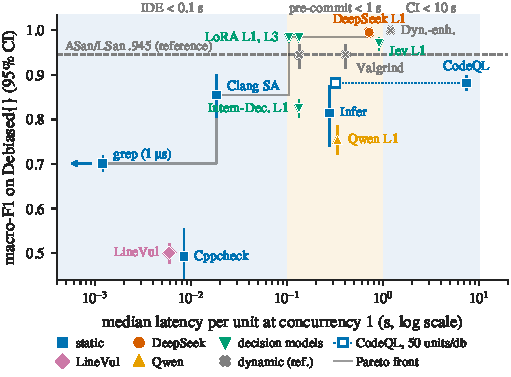
\includegraphics[width=\columnwidth]{figures/pareto.pdf}
\caption{Accuracy vs latency per unit at concurrency 1 (Table~\ref{tab:latency}), against the deployment budgets of an IDE ($<$0.1\,s), a pre-commit hook ($<$1\,s) and CI ($<$10\,s).
Vertical bars: 95\% CI. The hollow CodeQL marker is the amortized cost with 50 units per database.
grep (1\,\textmu s) is drawn at the left edge.}
\label{fig:pareto}
\end{figure}

% generated by figures/make_figures.py -- do not edit
% src: juliet_full/analysis/score.py on figures/latency_c1.csv (latency files listed there); juliet_full/llm/ledger.jsonl; decision_ft/runs/L?/fold?/train_log.jsonl
\begin{table}[t]
\centering
\caption{Latency per unit at concurrency 1 on the 300-unit latency sample (CodeQL per unit: 20 units; LineVul GPU: server side) as median and p90 in seconds, compile time included for dynamic tools, and marginal cost per 1,000 units: API price paid (off-peak DeepSeek, from the call ledger) or GPU-hours at the measured median. Sources: lane reports (a) static\_stage2, (b) gpu\_stage1, (c) gpu\_stage2, (d) decision\_ft\_stage2, (e) llm\_stage2d, (f) data\_stage4, recomputed from the latency files where they exist. $^\ddagger$Our LoRA training cost 4.6 GPU-hours in total (six adapters, RTX 3090).}
\label{tab:latency}
\scriptsize
\setlength{\tabcolsep}{3pt}
\begin{tabular}{@{}lrrlc@{}}
\toprule
Method & median & p90 & cost / 1k units & src \\
\midrule
grep & $<$0.001 & $<$0.001 & CPU & a \\
Cppcheck & 0.008 & 0.010 & CPU & a \\
Clang SA & 0.018 & 0.022 & CPU & a \\
Infer (Pulse) & 0.278 & 0.647 & CPU & a \\
CodeQL, 1 unit/db & 7.36 & 7.91 & CPU & a \\
CodeQL, 50 units/db & 0.318 & 0.334 & CPU & a \\
\midrule
LineVul (GPU) & 0.006 & 0.007 & 0.002 GPU-h & b \\
LineVul (CPU) & 0.088 & 0.124 & CPU & c \\
LoRA L1 (GPU) & 0.105 & 0.130 & 0.029 GPU-h & d \\
LoRA L3 (GPU)$^\ddagger$ & 0.133 & 0.148 & 0.037 GPU-h & d \\
Intern-Dec. L1 (GPU) & 0.132 & 0.149 & 0.037 GPU-h & c \\
Qwen L1 (GPU, vLLM) & 0.333 & 0.357 & 0.093 GPU-h & c \\
DeepSeek L1 (API) & 0.715 & 1.03 & \textyen0.397 & e \\
Jev L1 (API) & 0.907 & 0.931 & \$0.0345 & e \\
\midrule
ASan/LSan (ref.) & 0.134 & 0.209 & CPU & f \\
Valgrind (ref.) & 0.407 & 0.548 & CPU & f \\
Dynamic-enh.\ (ref.) & 1.19 & 2.20 & CPU & f \\
\midrule
\multicolumn{5}{@{}p{\linewidth}@{}}{DeepSeek L1/L2/L3/L4: \textyen0.397 / \textyen0.340 / \textyen0.268 / \textyen0.634; Jev L1/L2/L3: \$0.0345 / \$0.0641 / \$0.0367 per 1k} \\
\bottomrule
\end{tabular}
\end{table}


Fig.~\ref{fig:pareto} plots macro-F1 against median latency at concurrency 1 (Table~\ref{tab:latency}).
Bulk runs were concurrent, so their per-call times are not used.
Four methods form the Pareto front: grep, Clang SA (\res{x}{lat_clang_sa}\,s), our LoRA classifier
(\res{x}{lat_lora_L1}\,s on one RTX 3090) and DeepSeek L1 (\res{x}{lat_deepseek_L1}\,s over the API).
Clang SA is the only accurate analyzer inside the IDE budget.
LoRA sits on the IDE boundary and comes close to DeepSeek's accuracy at a seventh of its latency.
CodeQL needs \res{x}{lat_codeql}\,s per unit when it builds one database per unit
and \res{x}{lat_codeql_amortized}\,s when 50 units share a database.
That puts it in CI rather than in an editor.
Both API models fit a pre-commit hook.
They cost \textyen\res{x}{cost1k_deepseek_L1} (DeepSeek L1) and \$\res{x}{cost1k_jev_L1} (Jev L1) per 1,000 units.
All DeepSeek runs of the project cost \textyen\res{x}{cost_deepseek} and all Jev runs \$\res{x}{cost_jev}.
The local models need \res{x}{gpuh1k_lora_L1}--\res{x}{gpuh1k_qwen_L1} GPU-hours per 1,000 units.
Training the six LoRA adapters took \res{x}{ft_hours_total} GPU-hours.
Dynamic analysis is accurate and cheap per unit (ASan/LSan \res{x}{lat_asan_lsan}\,s including compilation).
However, it needs a harness that drives the leaking path, which a static setting does not have.

\subsection{RQ4: Robustness to never-executed frees}\label{sec:rq4}

\begin{figure}[t]
\centering
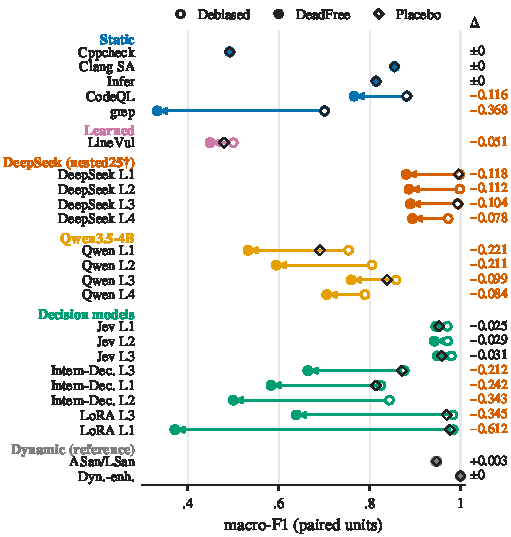
\includegraphics[width=\columnwidth]{figures/robust.pdf}
\caption{Paired macro-F1 on \Deb{} (hollow) and \Dead{} (filled) for the same units, with \Plac{} (diamond) as the control for inserting code at all.
$\Delta$ = \Dead{} $-$ \Deb. $^\dagger$DeepSeek on nested25 (\res{x}{n_nested25} units).}
\label{fig:robust}
\end{figure}

% generated by figures/make_figures.py -- do not edit
% src: juliet_full/analysis/score.py on layer1/, layer3/ (data/results/*/stress/) and placebo/ runs in generated/results_summary.json
\begin{table}[t]
\centering
\caption{Robustness to never-executed frees, paired on the same units. \Deb, \Dead: macro-F1; $\Delta$ = \Dead{} $-$ \Deb; $\Delta_{\mathrm{pl}}$ = \Plac{} $-$ \Deb; adj = $\Delta - \Delta_{\mathrm{pl}}$; flips: changed verdicts; lost: leaks found on \Deb{} and missed on \Dead; new FP: goods correct on \Deb{} and flagged on \Dead. $^\dagger$nested25 (664 units), else 2,656.}
\label{tab:robust}
\scriptsize
\setlength{\tabcolsep}{1.5pt}
\begin{tabular}{@{}lrrrrrrrr@{}}
\toprule
Method & \Deb{} & \Dead{} & $\Delta$ & $\Delta_{\mathrm{pl}}$ & adj & flips & lost & new FP \\
\midrule
\multicolumn{9}{@{}l}{\textit{Static analyzers and baselines}} \\
\quad grep & 0.701 & 0.333 & $-$0.368 & $\pm$0.000 & $-$0.368 & 1,755 & 1,155 & 0 \\
\quad Cppcheck & 0.493 & 0.493 & $\pm$0.000 & $\pm$0.000 & $\pm$0.000 & 0 & 0 & 0 \\
\quad Clang SA & 0.855 & 0.855 & $\pm$0.000 & $\pm$0.000 & $\pm$0.000 & 0 & 0 & 0 \\
\quad CodeQL & 0.882 & 0.766 & $-$0.116 & $\pm$0.000 & $-$0.116 & 309 & 309 & 0 \\
\quad Infer & 0.815 & 0.815 & $\pm$0.000 & $\pm$0.000 & $\pm$0.000 & 0 & 0 & 0 \\
\addlinespace[2pt]
\multicolumn{9}{@{}l}{\textit{Learned (zero-shot)}} \\
\quad LineVul & 0.501 & 0.449 & $-$0.051 & $-$0.021 & $-$0.031 & 576 & 43 & 257 \\
\addlinespace[2pt]
\multicolumn{9}{@{}l}{\textit{DeepSeek-V4.1-Flash}} \\
\quad DeepSeek L1$^\dagger$ & 0.998 & 0.881 & $-$0.118 & $-$0.003 & $-$0.115 & 78 & 25 & 53 \\
\quad DeepSeek L2$^\dagger$ & 0.998 & 0.887 & $-$0.112 & -- & -- & 76 & 19 & 56 \\
\quad DeepSeek L3$^\dagger$ & 0.994 & 0.890 & $-$0.104 & $\pm$0.000 & $-$0.104 & 73 & 15 & 56 \\
\quad DeepSeek L4$^\dagger$ & 0.973 & 0.895 & $-$0.078 & -- & -- & 66 & 37 & 22 \\
\addlinespace[2pt]
\multicolumn{9}{@{}l}{\textit{Qwen3.5-4B}} \\
\quad Qwen L1 & 0.754 & 0.533 & $-$0.221 & $-$0.063 & $-$0.158 & 959 & 9 & 674 \\
\quad Qwen L2 & 0.806 & 0.595 & $-$0.211 & -- & -- & 670 & 10 & 543 \\
\quad Qwen L3 & 0.858 & 0.760 & $-$0.099 & $-$0.020 & $-$0.079 & 385 & 13 & 305 \\
\quad Qwen L4 & 0.790 & 0.706 & $-$0.084 & -- & -- & 466 & 195 & 150 \\
\addlinespace[2pt]
\multicolumn{9}{@{}l}{\textit{Decision models}} \\
\quad Jev L1 & 0.971 & 0.946 & $-$0.025 & $-$0.018 & $-$0.007 & 119 & 67 & 26 \\
\quad Jev L2 & 0.972 & 0.942 & $-$0.029 & -- & -- & 136 & 78 & 29 \\
\quad Jev L3 & 0.980 & 0.949 & $-$0.031 & $-$0.021 & $-$0.010 & 119 & 79 & 22 \\
\quad Intern-Dec. L1 & 0.825 & 0.583 & $-$0.242 & $-$0.011 & $-$0.230 & 730 & 17 & 603 \\
\quad Intern-Dec. L2 & 0.844 & 0.500 & $-$0.343 & -- & -- & 812 & 14 & 741 \\
\quad Intern-Dec. L3 & 0.876 & 0.664 & $-$0.212 & $-$0.005 & $-$0.207 & 558 & 18 & 506 \\
\quad LoRA L1 & 0.984 & 0.372 & $-$0.612 & $-$0.008 & $-$0.604 & 1,267 & 1,234 & 30 \\
\quad LoRA L3 & 0.983 & 0.639 & $-$0.345 & $-$0.014 & $-$0.331 & 851 & 791 & 52 \\
\addlinespace[2pt]
\multicolumn{9}{@{}l}{\textit{Dynamic (reference, not ranked)}} \\
\quad ASan/LSan & 0.945 & 0.948 & +0.003 & +0.002 & +0.001 & 12 & 2 & 0 \\
\quad Dynamic-enh. & 1.000 & 1.000 & $\pm$0.000 & $\pm$0.000 & $\pm$0.000 & 0 & 0 & 0 \\
\bottomrule
\end{tabular}
\end{table}


\Dead{} adds frees under always-false guards and wraps every real free in an always-true guard.
\Plac{} inserts the same guards around a harmless print.
Fig.~\ref{fig:robust} and Table~\ref{tab:robust} give the paired changes.
The placebo deltas are small for every method except Qwen L1 (\res{qwen_L1-placebo}{d}),
so the \Dead{} deltas measure guard reasoning, not the edit itself.
The methods fail in two opposite ways.
\textbf{Trusting a dead free causes misses.}
grep loses all \res{grep-layer3}{lost} of its detections (\res{grep-layer3}{d}).
CodeQL loses \res{codeql-layer3}{lost} (\res{codeql-layer3}{d}): in these units its query accepts a never-executed free as a release.
Our LoRA classifier loses \res{lora_L1-layer3}{lost} with L1 input:
macro-F1 falls from \res{lora_L1-layer1}{macro} to \res{lora_L1-layer3}{macro} and leak recall to \res{lora_L1-layer3}{r}.
\textbf{Doubting a guarded real free causes false alarms.}
Qwen L1 adds \res{qwen_L1-layer3}{gained} false positives and Intern-Decision L1 adds \res{intern_L1-layer3}{gained},
while both still find almost every leak (recall \res{qwen_L1-layer3}{r} and \res{intern_L1-layer3}{r}).
The path-sensitive analyzers Clang SA and Infer do not change a single verdict (\res{clang_sa-layer3}{flips} and \res{infer-layer3}{flips} flips),
and neither does dynamic-enhanced, which executes the guards.
ASan/LSan changes \res{asan_lsan-layer3}{flips} verdicts, all on flow~12, whose path is random at run time.

DeepSeek loses \res{deepseek_L1-layer3}{d} (L1) to \res{deepseek_L3-layer3}{d} (L3) in both directions:
\res{deepseek_L1-layer3}{lost} lost detections and \res{deepseek_L1-layer3}{gained} new false positives for L1.
L4 is its most robust strategy (\res{deepseek_L4-layer3}{d}).
Its errors shift towards misses (\res{deepseek_L4-layer3}{fp} FP and \res{deepseek_L4-layer3}{fn} FN, against \res{deepseek_L1-layer3}{fp} and \res{deepseek_L1-layer3}{fn} for L1).
Jev is the most robust LLM-based detector (\res{jev_L1-layer3}{d} to \res{jev_L3-layer3}{d}).

% generated by figures/make_figures.py -- do not edit
% src: juliet_full/analysis/score.py on decision_ft/results/decision_ft/<layer>/L{1,3}_cv_v1.jsonl, unmerged_L*_fold*_v1.jsonl, qwen_readout_zeroshot/<layer>/L*_v1.jsonl
\begin{table}[t]
\centering
\caption{Our LoRA decision model (3-fold CV; every unit scored by the adapter that did not train on it) against the same base model and read-out head without LoRA (threshold chosen on dev). R: leak recall on \Dead. AUROC per fold 0/1/2 (one value for the single base model).}
\label{tab:lora}
\scriptsize
\setlength{\tabcolsep}{1.4pt}
\begin{tabular}{@{}lrrrrll@{}}
\toprule
 & \multicolumn{4}{c}{macro-F1 (R)} & \multicolumn{2}{c}{AUROC} \\
\cmidrule(lr){2-5}\cmidrule(l){6-7}
Variant & \Deb{} & \Dead{} & R & \Plac{} & \Deb{} & \Dead{} \\
\midrule
LoRA L1 & 0.984 & 0.372 & 0.041 & 0.976 & .999/.957/1.0 & .691/.677/.703 \\
LoRA L3 (+Clang) & 0.983 & 0.639 & 0.379 & 0.970 & .999/.981/1.0 & .911/.867/.888 \\
\addlinespace[2pt]
no LoRA, L1 & 0.703 & 0.619 & 0.989 & -- & 0.789 & 0.729 \\
no LoRA, L3 & 0.773 & 0.671 & 0.977 & -- & 0.862 & 0.820 \\
\addlinespace[2pt]
unmerged L1 & 0.984 & -- & -- & -- & .999/.956/1.0 & -- \\
unmerged L3 & 0.983 & -- & -- & -- & .999/.980/1.0 & -- \\
\bottomrule
\end{tabular}
\end{table}


\textbf{The LoRA shortcut} (Table~\ref{tab:lora}).
With the same base model and read-out head, the classifier without LoRA reaches only \res{readout_L1-layer1}{macro} on \Deb.
The adapter therefore learned almost all of the task.
Under cross-validation it scores \res{lora_L1-layer1}{macro} on \Deb, and the merged and unmerged weights agree on every unit
(\res{x}{unmerged_flips_L1} flips for L1, \res{x}{unmerged_flips_L3} for L3).
On \Dead{} it collapses: per-fold AUROC drops from
\res{x}{auroc_lora_L1_layer1_f0}/\res{x}{auroc_lora_L1_layer1_f1}/\res{x}{auroc_lora_L1_layer1_f2}
to \res{x}{auroc_lora_L1_layer3_f0}/\res{x}{auroc_lora_L1_layer3_f1}/\res{x}{auroc_lora_L1_layer3_f2}.
What it learned is ``a free is present'', not whether the free executes.
Adding the Clang SA evidence (L3 input) recovers part of the gap (\res{lora_L3-layer3}{macro}, recall \res{lora_L3-layer3}{r}).
Dev AUROC was saturated at 1.0, so checkpoints were chosen by dev loss, and dev data could not have revealed this failure.
% src: juliet_full/lane_reports/2026-11-23_decision_ft_stage2.md (dev AUROC 1.0, selection by dev loss)

% generated by figures/make_figures.py -- do not edit
% src: juliet_full/analysis/score.py on registry repeats in figures/methods.json; gpu/results/intern_decision/layer1/det50_L1_r2.jsonl; decision_ft/runs/endpoint/spot_check.json
\begin{table}[t]
\centering
\caption{Run-to-run variation on \Deb. Three runs (the main run and two repeats) on the repeat sample (eval $\cap$ repeat100); Jev was repeated on all 2,656 eval units. Agreement = share of units with the same verdict in all three runs.}
\label{tab:repeat}
\footnotesize
\begin{tabular}{@{}lrrl@{}}
\toprule
Model & units & agreement & macro-F1 per run \\
\midrule
DeepSeek L1 & 200 & 1.000 & 1.0/1.0/1.0 \\
DeepSeek L2 & 200 & 1.000 & 1.0/1.0/1.0 \\
DeepSeek L3 & 200 & 0.990 & 1.0/.990/.995 \\
Jev L1 & 2,656 & 0.989 & .971/.972/.971 \\
Jev L2 & 2,656 & 0.996 & .972/.972/.972 \\
Jev L3 & 2,656 & 0.995 & .980/.982/.980 \\
Qwen L1 & 200 & 0.985 & .745/.745/.755 \\
Qwen L2 & 200 & 0.995 & .822/.817/.822 \\
Qwen L3 & 200 & 0.985 & .830/.835/.835 \\
\midrule
Intern-Dec. L1 rerun & 50 & 1.000 & identical scores 50/50 \\
LoRA endpoint replay & 22 & 1.000 & max $|\Delta s|$ = 0.0 \\
\bottomrule
\end{tabular}
\end{table}


\textbf{Run-to-run variation} (Table~\ref{tab:repeat}).
DeepSeek gives the same verdict in all three runs for \res{x}{rep_DeepSeek_L1} (L1) to \res{x}{rep_DeepSeek_L3} (L3) of the repeat units,
and Jev for \res{x}{rep_Jev_L1}--\res{x}{rep_Jev_L2} of all eval units,
so single-run differences of a few units are noise.
Qwen agrees on \res{x}{rep_Qwen_L1}--\res{x}{rep_Qwen_L2} of the repeat units.
Intern-Decision reproduces its scores exactly in a rerun (\res{x}{intern_det_same}/\res{x}{intern_det_n} units),
and the LoRA endpoint replays the bulk scores exactly.
